\documentclass[7pt]{article}
\usepackage{amsmath}
\usepackage{graphicx}
\usepackage{caption}
\usepackage[landscape]{geometry}
\usepackage{multicol}
\usepackage{amssymb}
\usepackage{geometry}
 \geometry{
 a4paper,
 total={285mm,185mm},
 left=10mm,
 top=10mm,
 }

\setlength\columnseprule{0.5pt}
\setlength{\parindent}{0pt}
\graphicspath{ {images/} }


\begin{document}
\begin{multicols}{3}
	

\section{Kinematik}

\subsection{Allgemeine Zusammenh{\"a}nge}
\mbox{} \\
\[Weg \mathrel{\mathop{\rightleftarrows}^{\mathrm{ableiten}}_{\mathrm{integrieren}}} Geschwindigkeit \mathrel{\mathop{\rightleftarrows}^{\mathrm{ableiten}}_{\mathrm{integrieren}}} Beschleunigung\]
\newline

\begin{center}
	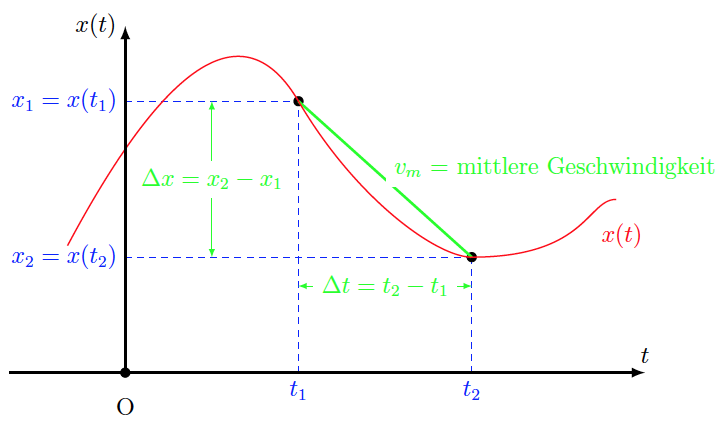
\includegraphics[width=200pt]{images/kinematik}
\end{center}

\paragraph{Verschiebung:}
\begin{equation*}
	{\Delta}x = x_2 - x_1 = x(t_2) - x(t_1) 
\end{equation*}

\paragraph{Mittlere Geschwindigkeit:}
\begin{equation*}
	V_m = \frac{{\Delta}x}{{\Delta}t} =  \frac{x_2 - x_1}{t_2 - t_1} = \frac{x(t_2) - x(t_1)}{t_2 - t_1}
\end{equation*}

\paragraph{Momentane Geschwindigkeit}\mbox{} \\
\begin{equation*}
	v(t) = \frac{dx}{dt}	 \>\>oder\>\> V = at
\end{equation*}

\paragraph{Beschleunigung}\mbox{} \\
\begin{equation*}
	a_m = \frac{{\Delta}v}{{\Delta}t} \>\>oder\>\> a = \frac{V}{t}
\end{equation*}

\begin{equation*}
a(t) = \frac{dv}{dt} = \frac{d}{dt} \left(\frac{dx}{dt}\right) = \frac{d^2x}{dt^2}
\end{equation*}


\subsection{Integration der Bewegung}
\begin{equation*}
	v(t) = \frac{dx}{dt} \>\> \rightarrow \>\> dx = v(t)dt
\end{equation*}
\begin{center}
dx =  Weg innerhalb des Zeitintervalls dt\newline
\end{center}

\begin{equation*}
	x(t) = \int_{t_0}^{t}v(t)dt' = \int_{x(t_0)=x_0}^{x(t)}dx = x(t) - x_0
\end{equation*}
\newline

Schlussendlich folgt daraus:
\begin{equation*}
	x(t) = \int_{t_0}^{t}v(t')dt' + x_0
\end{equation*}
\begin{equation*}
	v(t) = \int_{t_0}^{t}a(t')dt' + v_0
\end{equation*}

$x(t)$ ist die Stammfunktion von $v(t)$ \\
$x_0$ entspricht dem Startpunkt \\
$v_0$ entspricht der Startgeschwindigkeit\newline
\newline
\newline
Falls die Bewegung gleichf{\"o}rmig und geradlinig \\
($v(t) = konst. \Rightarrow a(t) = 0$) gilt:\newline
\begin{equation*}
	x(t) = x_0 + v_0(t - t_0)
\end{equation*}
\newline
Falls die Bewegung gleichf{\"o}rmig beschleunigt und geradlinig ($a(t) = a_0 = konst.$) gilt: \newline
\begin{equation*}
\begin{split}
		v(t)& = v_0 + a_0(t - t_0)\\
	x(t)& = x_0 + v_0(t - t_0) + \frac{1}{2}a_0(t - t_0)^2
\end{split}
\end{equation*}
\newline

Spezialfall: $x_0 = v_0 = t_0 = 0$ \newline
\begin{equation*}
\begin{split}
	x(t)& = \frac{1}{2}a_0t^2 \\
	v(t)& = a_0t \\
	a(t)& = a_0
\end{split}
\end{equation*}

\subsection{Freier Fall / Gravitation}
In der N{\"a}he der Erdoberfl{\"a}che f{\"u}hlt jeder K{\"o}per, ubabh{\"a}ngig von seinem Gewicht, dieselbe Beschleunigung (wenn der Luftwiderstand vernachl{\"a}ssigt wird).

\begin{equation*}
	h = \frac{1}{2}a_0t^2 = \frac{1}{2}gt^2
\end{equation*}
\begin{equation*}
\Rightarrow t = \sqrt{\frac{2h}{g}}
\end{equation*}
mit Fallh{\"o}he $h$ und Fallzeit $t$.
\newline

$Hinweis:$ Es existiert eine Grenzgeschwindigkeit, da der Luftwiderstand mit der Geschwindigkeit (quadratisch) des K{\"o}rpers zu nimmt.


\subsection{Bewegung in mehreren Dimensionen}
\begin{equation*}
r = r(t) = x(t) e_x + y(t) e_y
\end{equation*}
In Kugelkoordinaten:
\begin{equation*}
r = r(t)e_r(t)
\end{equation*}

\paragraph{Geschwindigkeit:}
\begin{equation*}
v(t) = v_x(t)e_x + v_y(t)e_y = \frac{dx}{dt}e_x +\frac{dy}{dt}e_y 
\end{equation*}

In Kugelkoordinaten:
\begin{equation*}\label{eq:dN}
v(t) = \frac{dr}{dt}e_r + r\frac{de_r}{dt}e_y = \underbrace{\frac{dr}{dt}e_r}_{\substack{1}} + \underbrace{r\frac{d{\varphi}}{dt}e_{\varphi}}_{\substack{2}}
\end{equation*}

$1:$ radiale Geschwindigkeit $V_r$ \newline
$2:$ Winkelgeschwindigkeit $V_{\varphi}$ senkrecht zu $e_r$ in Richtung $e_{\varphi}$
\newline
\newline
Vereinfacht dargestellt:

$V(t) = V_r + V_{\varphi}$
$\>\>\>\>$ mit 
$V_{\varphi} = r\frac{d{\varphi}}{dt}e_{\varphi} = r{\omega}e_{\varphi}$




\subsection{Bahnkurve beim Ballwurf}

Zur Zeit $t_{max}$ erreicht die Kugel den h{\"o}chsten Punkt ihrer Bahnkurve. In diesem Punkt verschwindet die vertikale Geschwindigkeit:
\begin{equation*}
	t_{max} = \frac{v_{0y}}{g}
\end{equation*}

Die maximale H{\"o}he der Kugel ist:
\begin{equation*}
	y_{max} = y_0 + \frac{{v_{0y}}^2}{2g}
\end{equation*}

\subsection{Gleichf{\"o}rmige Kreisbewegung}

\begin{equation*}
	\varphi(t) = \omega t
\end{equation*}

mit Winkelgeschwindigkeit $\omega$ und Periode $T$:
\begin{equation*}
	\varphi(T) = 2 \pi \Rightarrow T = \frac{2 \pi}{\omega}
\end{equation*}

\subsubsection{Geschwindigkeitsvektor}
Betrag: $|\vec{v}| = r \omega = konst.$ \newline
Die Richtung der Geschwindigkeit ist senkrecht zum Ortsvektor.

\subsubsection{Beschleunigungsvektor = Zentripetalbeschleunigung}
Zeigt in Richtung Zentrum des Kreises mit Betrag: $\vec{a} = r \omega ^2 = \frac{v^2}{r}$


\begin{center}
	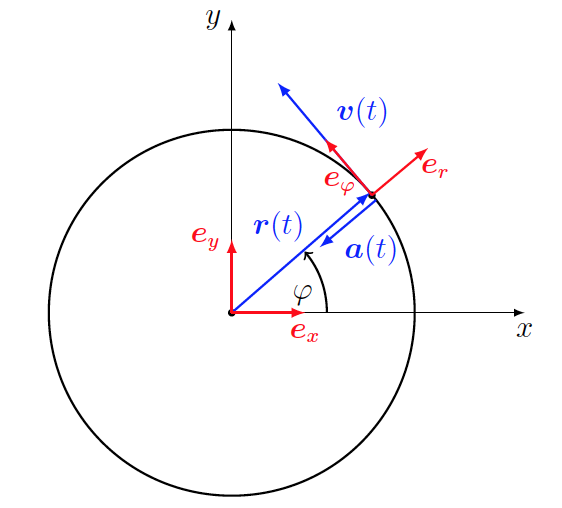
\includegraphics[width=200pt]{images/beschleunigung_radial}
\end{center}


\end{multicols}
\end{document}